\documentclass[main]{subfiles}

\begin{document}


\chapter{Diseño del controlador}
\label{chap:control}

Dentro del ``mundo'' del control lineal, existen diversas t\'ecnicas que nos permiten alcanzar el objetivo trazado de lograr que el cuadric\'optero siga alguna de las trayectorias espec\'ificadas en el cap\'itulo \ref{chap:linealizacion}. Algunas de las t\'ecnicas m\'as utilizadas se centran en el diseño de controladores PID\footnote{Proporcional, integral y derivativo} o LQR\footnote{Linear quadratic regulator}. Ambas t\'ecnicas presentan ventajas y desventajas. En el trabajo realizado en \cite{bib:quadrotor-bible} se propone el control de un cuadric\'optero utilizando un controlador PID. La gran mayor\'ia de controladores en aplicaciones industriales son de este tipo, la principal ventaja que presentan es que se trata de un diseño que tiene una estructura simple y es adecuado para la gran mayor\'ia de procesadores ya que el costo computacional del mismo es pr\'acticamente nulo. El concepto principal es que la señal de entrada a la planta es una funci\'on del error entre el estado deseado y el estado estimado.
\begin{equation}
u(t) = K_pe(t)+K_I\int_0^t e(\tau) d\tau +K_d\frac{de(t)}{dt}
\end{equation}

donde $e(t) = X_d-\hat{X}$, siendo $X_d$ el vector de estados deseado.\\

Es fundamental en esta t\'ecnica de control la determinaci\'on de las constantes. En \cite{bib:quadrotor-bible} se limitan las trayectorias a trayectorias de hovering. En ese supuesto, se realizan algunas aproximaciones que permiten reducir el sistema f\'isico a las siguientes ecuaciones
\begin{equation}
\left(
\begin{array}{c}
\ddot{z}\\
\ddot{\psi}\\
\ddot{\varphi} \\
\ddot{\theta}
\end{array}\right)
=\left(\begin{array}{c}
g+(\cos\varphi\cos\psi)\frac{U_1}{M}\\
 \frac{U_2}{I_{xx}} \\
 \frac{U_3}{I_{yy}} \\
 \frac{U_4}{I_{zz}} \\
\end{array}\right)
\end{equation}

Donde $U_1, U_2, U_3$ y $U_4$ son combinaciones lineales de los cuadrados de las velocidades angulares de cada motor. En este caso se puede tratar cada variable por separado, ya que cada variable es afectada por una sola entrada, siendo relativamente sencillo determinar las constantes $K_p, K_I$ y $K_d$ en funci\'on de donde se desea ubicar los polos del sistema realimentado. Con esta estrategia se pierde la posibilidad de controlar las otras 8 variables de estado, limit\'andose entonces a un cuadric\'optero que puede realizar exclusivamente movimientos en la direcci\'on vertical y giros en torno a su eje vertical.\\

Si se intenta controlar el sistema de inter\'es en este trabajo utilizando esta t\'ecnica, nos enfrentar\'iamos al problema de determinar al menos una matriz de realimentaci\'on (si trabajamos solamente con un controlador proporcional). Dicha matriz, debe ser de $12\times4$, es decir que se deben determinar los 48 elementos de la matriz de forma de lograr que la respuesta del sistema sea la deseada. Esta tarea no resulta sencilla, ya que es extremadamente dificultoso comprender exactamente la influencia de cada par\'ametro de la matriz de realimentaci\'on en la ubicaci\'on de los polos en el sistema realimentado incluso para asegurar algo elemental y necesario como la estabilidad del sistema.\\

Por dicho motivo se opto por explorar el camino propuesto por otros trabajos como \cite{bib:lqr-discreto}, donde la t\'ecnica elegida para realizar el control del cuadric\'optero es LQR.


\section{Conceptos generales sobre LQR}

Consideremos el sistema realimentado de la figura \ref{fig:bloque}, con $X(t)\in \mathcal{M}_{n\times1}$ el vector de estados del sistema y $u(t)\in \mathcal{M}_{m\times1}$ las entradas. $r$ es el setpoint del cual, multiplicando por dos matrices adecuadas pueden obtenerse los valores deseados de entrada $U^*$ y de las variables de estado $X^*$. El objetivo que nos planteamos es el de obtener una matriz de realimentaci\'on K para el sistema utilizando la t\'ecnica de LQR. 

\begin{figure}[h!]
	\centering
	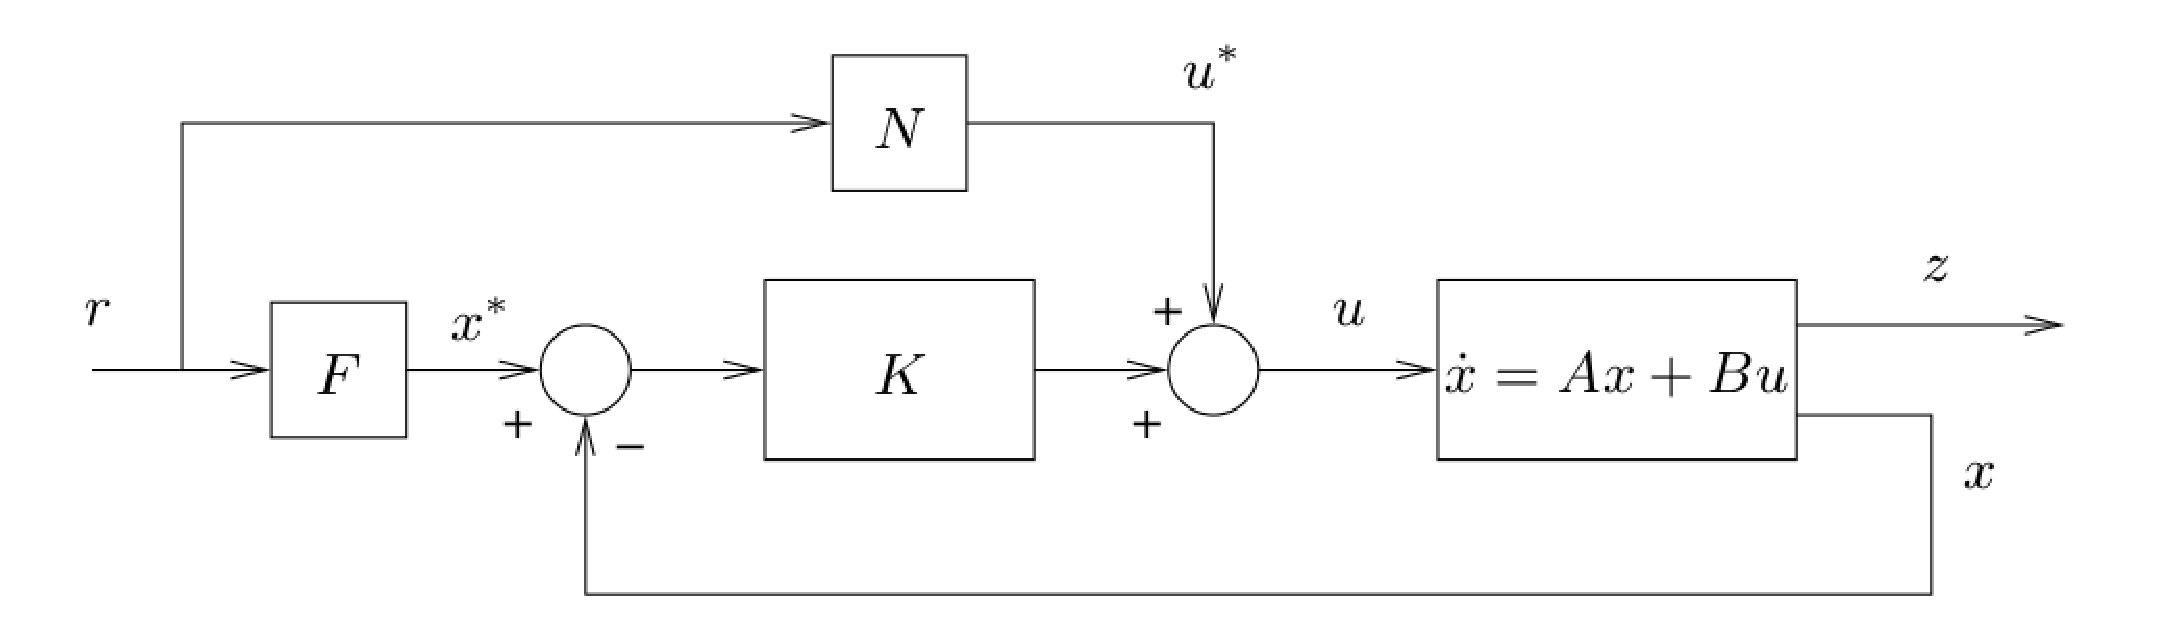
\includegraphics[width=0.7\textwidth]{./pics_control/bloque.pdf}
	\caption{Sistema realimentado}
	\label{fig:bloque}
\end{figure}
 
El problema de encontrar un regulador \'optimo de horizonte infinito puede plantearse de la siguiente forma: se trata de encontrar la matriz de transferencia $C(s)$ que minimice la siguiente funci\'on de costo:

\begin{equation}
\label{eq:lqr}
J_{LQR} = \int_{0}^{\infty}  X'(t)Q X(t)+U'(t)RU(t)dt
\end{equation}

Donde $Q$ y $R$ son matrices sim\'etricas definidas positivas de dimensiones $n\times n$ y $m\times m$ respectivamente. 

El primer t\'ermino de la integral corresponde a la energ\'ia de los estados controlados y el segundo a la energ\'ia de la señal de control. En funci\'on de como se escogen las matrices $Q$ y $R$, se obtienen resultados distintos. Por ejemplo si la norma de $Q$ es pequeña la forma m\'as efectiva de reducir $J_{LQR}$ es utilizar señales de control de norma pequeña a expensas de tener grandes variaciones en los estados controlados. Si bien existen diversos m\'etodos para determinar las matrices $Q$ y $R$, gran parte del trabajo es iterativo y se realiza a ensayo y error\\  

En la versi\'on de realimentaci\'on de estados del problema LQR se asume que se disponen de medidas de todas las variables del vector de estados. En este caso, el controlador \'optimo LQR es una matriz de ganancia K tal que:
\begin{equation}
U(t)-U^*(t) = -K(X(t)-X^*(t))
\end{equation}

Donde $K\in\mathcal{M}_{m\times n}$. Para el caso bajo an\'alisis se tiene que: 

\begin{equation}
K = R^{-1}B^TP
\end{equation}

Donde P es la soluci\'on a la ecuaci\'on algebraica de Riccati.

La propiedad escencial del controlador LQR es que la respuesta del sistema en lazo cerrado es asint\'oticamente estable, es decir que la parte real de los valores propios de la matriz $A-BK$ es negativa, mientras se cumplan las siguientes condiciones:

\begin{itemize}
\item El sistema es controlable
\item El sistema es observable
\end{itemize}

\section{Consideraciones particulares respecto del sistema a controlar}

Como se explico en cap\'itulos anteriores, se tienen una nueva estimaci\'on del vector de estados cada $10 ms$, lo cual nos permite realizar acciones de control con esta misma tasa de muestreo. De acuerdo a las constantes de tiempo que involucra el sistema f\'isico se puede afirmar que es un tiempo de acci\'on adecuado para trabajar.\\
% A modo de ejemplo consideremos la variable $\omega_{q_z}$. De acuerdo a las velocidades angulares de los motores que se utilizar\'an ($109 rads^{-1} < w_i < 387 rads^{-1})$ y suponiendo que nos encontramos trabajando a la velocidad angular de equilibrio ($334.28 rads^{-1}$ La aceleraci\'on angular m\'axima que puede darse es de $20.2 rad s^{-2}$. En el tiempo de muestreo implica un cambio en la velocidad angular de $11.5 ^{\circ} s^{-1}$ y un cambio en el \'angulo de Yaw de $0.058^{\circ}$. Estas pequeñas variaciones nos indican que el tiempo de acci\'on escogido es adecuado. Esto ser\'a confirmado posterioremente con las simulaciones realizadas. \\

Al tener un tiempo de respuesta r\'apido (en relaci\'on a las constantes del sistema) se podr\'ia resolver el problema utilizando la t\'ecnica de control LQR pensando en un sistema continuo, por m\'as que nuestro sistema sea discreto. Sin embargo los algor\'itmos de determinaci\'on de la soluci\'on a la ecuaci\'on algebraica de Ricatti m\'as sencillos que se encontraron corresponden a la soluci\'on de la formulaci\'on discreta del problema planteado en \ref{eq:lqr}. Por otra parte, dicha formulaci\'on corresponde al caso en el cual se trabaja con un horizonte infinito, es decir se busca alcanzar un determinado punto de operaci\'on y el setpoint no ser\'a modificado. Estrictamente, esta no es la situaci\'on en la cual nos encontramos dado que es de inter\'es concatenar diversas trayectorias, por ende el punto de operaci\'on s\'i debe ser modificado, sin embargo se puede suponer que cada trayectoria se realizar\'a por un tiempo ampliamente superior al tiempo del transitorio entre dos trayectorias. Por dicho motivo, aproximar el problema a un problema de horizonte infinito es acertado ya que simplifica enormemente la formulaci\'on del problema.

\subsection{Discretizaci\'on del sistema}

Como se explic\'o en el cap\'itulo \ref{chap:linealizacion} se trabjar\'a con tres tipos de trayectoria: hovering, vuelos en linea recta y c\'irculos. En cada uno de estos casos tenemos un sistema lineal de la forma 
\begin{equation}
\dot{X} = A X + BU
\end{equation}
 
La forma que toma el sistema continuo al ser convertido a tiempo discreto es: 
\begin{equation}
X_{k+1} = \Phi X_k + \Gamma U_k
\end{equation}
donde:
\begin{equation}
\Phi = e^{AT_s} \quad \Gamma = \int_0^{T_s} e^{A s} ds B
\end{equation}
Estas relaciones surgen de discretizar el sistema considerando muestreadores de \'orden cero. Por m\'as detalles de este proceso puede consultarse \cite{bib:hakas}.\\

El problema de encontrar un regulador \'optimo tambi\'en puede ser planteado en un sisetma discreto si reescribimos la ecuaci\'on \ref{eq:lqr}. 
\begin{equation}
\label{eq:dlqr}
J_{DLQR} = \sum_0^\infty X_k^T Q X_k + U_k^T R U_k
\end{equation}

En el trabajo realizado en \cite{bib:lqr-discreto} se propone un algoritmo iterativo para obtener la matriz de realimentaci\'on que minimiza $J_{DLQR}$. Debido a las pequeñas diferencias encontradas entre este algor\'itmo y la funci\'on \emph{lqrd} de \emph{MatLab}  se opt\'o por reproducir exactamente este \'ultimo.

\subsection{Agregado de integradores}

El esquema de la figura \ref{fig:bloque} funciona a la perfecci\'on solamente en el caso en que la caracterizaci\'on del sistema sea perfecta. Los valores de setpoint fueron determinados anal\'iticamente en funci\'on de los par\'ametros determinados, de forma que por ejemplo, para la trayectoria de hovering la velocidad angular de los motores es aquella que produce una fuerza igual al peso del sistema. Errores en la caracterizaci\'on del sistema llevan a que el punto (o trayectoria) de equilibrio no sea alcanzable. Supongamos que el valor de $\omega^*$ para la trayectoria de hovering es inferior al realmente necesario para mantener al sistema en un punto. Supongamos adem\'as que inicialmente $X = X^*$. En este caso la entrada al sistema es la velocidad angular $\omega^*$, sin embargo estamos suponiendo que esta fuerza no es suficiente para mantener al sistema en equilibrio, por lo tanto la posici\'on vertical disminuye. La realimentaci\'on proporcional produce un aumento en la velocidad angular de los motores hasta que para cierto valor de altura la entrada al sistema es aquella que produce el equilibrio. En este caso se obtiene un nuevo punto de equilibrio distinto al deseado. En el ejemplo considerado se obtiene una altura inferior a la deseada. \\

Realizando diversas pruebas se ha comprobado que seg\'un el nivel de bater\'ia disponible un mismo comando $I^2C$ corresponde a distintos valores de velocidad angular. Para resolver este problema se plantea el camino de medir el voltaje en la bater\'ia durante el vuelo, sin embargo este camino no parece pr\'actico ya que se deber\'ia caracterizar la relaci\'on entre velocidad angular y comando $I^2C$ para todo el rango de voltajes en que la bater\'ia puede operar. Este camino no parece pertinente, quedando incluso sujeto a la exactitud con la cual se realizan las medidas.\\

Surge entonces la necesidad de agregar al controlador cierta robustez frente a errores de caracterizaci\'on del sistema o frente a variaciones del mismo, por ejemplo la tensi\'on de la bater\'ia o un cambio en la masa del sistema\footnote{Para realizar pruebas se disponen de bater\'ias de diverso tamaño (y peso), no parece pr\'actico modificar constantemente la masa del sistema seg\'un la bater\'ia con la que se realiza una determinada prueba.} Esto \'ultimo es fundamental si se planea utilizar el cuadric\'optero por ejemplo para transportar alguna carga \'util.\\

%TODO no existe la fig:bloque2
El camino a explorar es el de agregar un bloque integrador. El esquema de controlador es ahora el de la figura \ref{fig:bloque2}. Para explicar la utilidad del mismo, continuaremos trabajando con el ejemplo de una trayectoria de hovering en la cual $\omega^*$ est\'a subestimado. En dichas condiciones se obtiene un nuevo punto de equilibro con altura inferior a la deseada. Si realimentamos la integral de la diferencia de altura tenemos una entrada que aumenta con el tiempo hasta que la diferencia de altura sea cero. En este punto el t\'ermino correspondiente a la integral de la diferencia de altura se mantiene constante en un valor positivo y el t\'ermino correspondiente a la realimentaci\'on proporcional es cero, compensando el error en el modelado.\\

El agregado de un bloque integrador lo podemos entender como una ampliaci\'on del vector de estados. La salida del bloque integrador verifica que $\dot{X}_I = X$. Donde $X_I$ corresponde a los estados integrados. La din\'amica del sistema puede ser escrita de la siguiente forma:
\begin{equation}
\label{eq:integrador}
\left(\begin{array}{c}
\dot{X}\\
\dot{X}_I
\end{array}\right) = \left( \begin{array}{cc}
A & 0\\
Id & 0
\end{array}\right)\left(\begin{array}{c}
X\\
X_I
\end{array}\right) + \left(\begin{array}{c}
B\\
0
\end{array}\right)U
\end{equation}  
 
En la ecuaci\'on \ref{eq:integrador} lo que se obtiene es un nuevo sistema lineal de mayor dimensi\'on. Lo que buscaremos ahora es encontrar una matriz de realimentaci\'on para el sistema \ref{eq:integrador} buscando minimizar la funci\'on de costos definida en \ref{eq:dlqr}.

\section{Controlabilidad y observabilidad}

Los conceptos de controlabilidad y observabilidad son fundamentales para asegurar la estabilidad del sistema en lazo cerrado controlado con la t\'ecnica de LQR.\\

Sea el sistema lineal representado por la ecuaci\'on \ref{eq:sis_lin}:
\begin{equation}
\label{eq:sis_lin}
\begin{array}{c}
\dot{X} = AX+BU \\
Y = CX+DU
\end{array}
\end{equation}
donde $A \in \mathcal{M}_{n \times n}$, $B \in \mathcal{M}_{n \times m}$, $C \in \mathcal{M}_{p \times n}$ y $D \in \mathcal{M}_{p \times m}$.\\

Consideremos la matrices $S\in \mathcal{M}_{n \times nm}$  definida como:
\begin{equation}
\label{eq:contr}
S = [B \quad AB \quad A^2B \quad ...\quad A^{n-1}B]
\end{equation}

El sistema es controlable si y solo si el rango de S es n. 

Consideremos la matriz $V\in \mathcal{M}_{pn \times n}$ definida como:
\begin{equation}
\label{eq:obs}
V=
\left[
\begin{array}{c}
 CA\\
CA^2\\
.\\
.\\
.\\
CA^{n-1}
\end{array}\right]
\end{equation}

El sistema es observable si y solo si el rango de V es n.\\

El sistema bajo estudio es originalmente no lineal. En el cap\'itulo \ref{chap:linealizacion} se estudi\'o en torno a que tipos de trayectorias se puede aproximar el problema de controlar el cuadric\'optero por el problema de controlar un sistema lineal invariante en el tiempo. Si bien no todas las trayectorias son posibles, el conjunto de trayectorias es infinito. Notar que por ejemplo dos vuelos en l\'inea recta a dos velocidades distintas son, en realidad, dos trayectorias distintas. Evidentemente, es imposible evaluar las condiciones de controlabilidad y observabilidad para todos los casos. Sin embargo, se puede evaluar en algunas trayectorias y confiar en que para las trayectorias no testeadas el resultado sea el mismo.\\

En una primer aproximaci\'on se analizaron diversas trayectorias para el sistema lineal sin los estados agregados correspondientes a la inclusi\'on de integradores. Las matrices de controlabilidad y observabilidad para todas las trayectorias testeadas son de rango 12. Esto implica que los controladores que surgen de la t\'ecnica de control LQR son estables. Sin embargo es de inter\'es, por los motivos presentados en la secci\'on anterior, poder agregar al controlador una dependencia del pasado (integradores), lo nos lleva a cuestionarnos que estados integrados pueden ser incluidos en el sistema manteniendo la condici\'on de controlabilidad. La condici\'on de observabilidad se cumple trivialmente ya que siempre se tiene una estimaci\'on de las integrales de los estados. \\

Los \'unicos estados que pueden integrarse sin perder la controlabilidad del sistema son las tres posiciones ($x,y,z$) y el \'angulo de Yaw ($\theta$). En resumen, el vector de estados controlados es el siguiente:

\begin{equation}
\label{eq:controled}
X = \left(\begin{array}{c}
x,y,z,\psi,\varphi,\theta,v_{q_x},v_{q_y},v_{q_z},\omega_{q_x},\omega_{q_y},\omega_{q_z},x_I,y_I,z_I,\theta_I
\end{array}\right)^T
\end{equation}

\section{Matriz de realimentaci\'on}

Como se explic\'o anteriormente, la matriz de realimentaci\'on es obtenida num\'ericamente gracias al algor\'itmo presentado en \cite{bib:lqr-discreto}. Dicha matriz depende del sistema lineal con el cual se representa cada trayectoria. Por lo tanto para cada trayectoria tendremos que calcular una nueva matriz de realimentaci\'on. Lo fundamental es entonces determinar adecuadamente las matrices Q y R presentadas en \ref{eq:dlqr} de forma de obtener trayectorias adecuadas. Estas matrices fueron determinadas en forma iterativa, modificando los par\'ametros hasta obtener un comportamiento satisfactorio en cuanto a tiempos de respuesta y robustez.\\

Se entiende que los par\'ametros fundamentales a controlar son los \'angulos de Euler, si el control sobre estos no se hace en forma r\'apida la performance del sistema puede verse afectada.  Las condiciones de vuelo determinadas dependen de que los \'angulos de Pitch y de Roll se encuentren perfectamente ajustados. Consideremos la condici\'on de hovering a modo de ejemplo, si estos \'angulos no son nulos se tiene un sistema que acelera indefinidamente en alguna direcci\'on. Por lo tanto parece importante darle un peso superior al control de estas variables de estado respecto a las restantes. Las matrices de realimentaci\'on se construyen a partir de:

\begin{equation}
\label{eq:Q}
Q = \left(\begin{array}{cccccccccccccccc}
1 & 0 & 0 & 0 & 0 & 0 & 0 & 0 & 0 & 0 & 0 & 0 & 0 & 0 & 0 & 0\\
0 & 1 & 0 & 0 & 0 & 0 & 0 & 0 & 0 & 0 & 0 & 0 & 0 & 0 & 0 & 0\\
0 & 0 & 1 & 0 & 0 & 0 & 0 & 0 & 0 & 0 & 0 & 0 & 0 & 0 & 0 & 0\\
0 & 0 & 0 & 1e3 & 0 & 0 & 0 & 0 & 0 & 0 & 0 & 0 & 0 & 0 & 0 & 0\\
0 & 0 & 0 & 0 & 1e3 & 0 & 0 & 0 & 0 & 0 & 0 & 0 & 0 & 0 & 0 & 0\\
0 & 0 & 0 & 0 & 0 & 1e3 & 0 & 0 & 0 & 0 & 0 & 0 & 0 & 0 & 0 & 0\\
0 & 0 & 0 & 0 & 0 & 0 & 1 & 0 & 0 & 0 & 0 & 0 & 0 & 0 & 0 & 0\\
0 & 0 & 0 & 0 & 0 & 0 & 0 & 1 & 0 & 0 & 0 & 0 & 0 & 0 & 0 & 0\\
0 & 0 & 0 & 0 & 0 & 0 & 0 & 0 & 1 & 0 & 0 & 0 & 0 & 0 & 0 & 0\\
0 & 0 & 0 & 0 & 0 & 0 & 0 & 0 & 0 & 1 & 0 & 0 & 0 & 0 & 0 & 0\\
0 & 0 & 0 & 0 & 0 & 0 & 0 & 0 & 0 & 0 & 1 & 0 & 0 & 0 & 0 & 0\\
0 & 0 & 0 & 0 & 0 & 0 & 0 & 0 & 0 & 0 & 0 & 1 & 0 & 0 & 0 & 0\\
0 & 0 & 0 & 0 & 0 & 0 & 0 & 0 & 0 & 0 & 0 & 0 & 1 & 0 & 0 & 0\\
0 & 0 & 0 & 0 & 0 & 0 & 0 & 0 & 0 & 0 & 0 & 0 & 0 & 1 & 0 & 0\\
0 & 0 & 0 & 0 & 0 & 0 & 0 & 0 & 0 & 0 & 0 & 0 & 0 & 0 & 1 & 0\\
0 & 0 & 0 & 0 & 0 & 0 & 0 & 0 & 0 & 0 & 0 & 0 & 0 & 0 & 0 & 1\\
\end{array}\right)
\end{equation}

\begin{equation}
\label{eq:R}
R = \left(\begin{array}{cccc}
0.1 & 0 & 0 & 0\\
0 & 0.1 & 0 & 0\\
0 & 0 & 0.1 & 0\\
0 & 0 & 0 & 0.1\\
\end{array}\right)
\end{equation}

\end{document}